\nocite{*}
\documentclass[12pt,a4paper]{article}
\usepackage[left=1.9cm, right=1.9cm, top=2.5cm, bottom=2.5cm]{geometry}
\usepackage[onehalfspacing]{setspace}
\usepackage[utf8]{inputenc}
\usepackage{ngerman}
\usepackage{bibgerm}
\usepackage{fancyhdr}
\setlength\parindent{0pt}

\usepackage{graphicx}
\renewcommand{\listfigurename}{Abbildungsverzeichnis}
\renewcommand{\listtablename}{Tabellenverzeichnis}
\usepackage{subfig}
\usepackage{wrapfig}
\usepackage{caption}
\usepackage{sidecap}
\usepackage{tikz}
\usetikzlibrary{calc}
\usetikzlibrary{shapes,arrows}
\usetikzlibrary{arrows.meta}
\usepackage{environ}
\usepackage{tikz-3dplot}
\usepackage{import}
\usepackage{calc}
\usepackage{pgfmath}
\usepackage{ifthen}
\usepackage{pgfplots}
\usepgfplotslibrary{fillbetween}
\usepackage{amsmath}
\usepackage{mathtools}
\DeclarePairedDelimiter\abs{\lvert}{\rvert}
\usepackage{makecell}
\usepackage{xr}
\usepackage{xurl}
\usepackage{footnote}
\usepackage[perpage, hang]{footmisc}
\usepackage{tablefootnote}
\usepackage{tabularx}
\usepackage{textcomp}
\usepackage[section]{placeins}
\usepackage[ngerman]{hyperref}
\usepackage[ngerman]{cleveref}
\setlength\footnotemargin{10pt}
\newcommand{\captionref} [1]{\textit{\nameref{#1}}}
\newcommand{\tableref} [1]{\textit{Tabelle \ref{#1}}}
\usepackage{listings}
\usepackage{chngcntr}
\usepackage{lipsum}
\usepackage{color, colortbl}
\usepackage{multirow}
\usepackage{float}
\usepackage[export]{adjustbox}
\newfloat{Ausschnitt}{htbp}{loa}
\newcolumntype{x}[1]{>{\centering\arraybackslash}p{#1}}
\usepackage{standalone}
\usepackage{blindtext}
\usepackage{pdfpages}


%define book numbering:
\def\frontmatter{%
    \pagenumbering{Roman}
    \setcounter{page}{1}
    \renewcommand{\thesection}{\Roman{section}}
}%

\def\mainmatter{%
    \pagenumbering{arabic}
    \setcounter{page}{1}
    \setcounter{section}{0}
    \renewcommand{\thesection}{\arabic{section}}
}%

\def\backmatter{%
    \setcounter{section}{0}
    \renewcommand{\thesection}{\Alph{section}}
}%

\tikzset{%
  block/.style    = {draw, thick, rectangle, minimum height = 3em,
    minimum width = 3em},
  sum/.style      = {draw, circle, node distance = 1.5cm}, % Adder
  input/.style    = {coordinate}, % Input
  output/.style   = {coordinate}, % Output
   base/.style = {rectangle, rounded corners, draw=black, minimum width=2cm, minimum height=1cm, text centered}
}

\begin{document}

    \counterwithout{figure}{section}
    \counterwithout{table}{section}
    \counterwithin{lstlisting}{section}
    \counterwithout{equation}{section}

    %Kopfzeile und Fußzeile
    \pagestyle{fancy}
    \fancyhf{}
    \lhead{Physik-Praktikum}
    \rhead{Versuche mit der schiefen Ebene}
    \lfoot{Hochschule Bielefeld, Fachbereich IuM}
    \cfoot{\thepage}
    \renewcommand{\headrulewidth}{0pt}

    \author{}

\begin{titlepage}
    \begin{center}
        
\includegraphics[width=7cm]{images/HSBI-Logo.png}\\ [10ex]
        \LARGE{\textbf{Versuchsbericht zum Thema}}\\[3ex]
        \huge{\textbf{Versuche mit dem mathematischen Pendel}}\\[20ex]
        \normalsize{}
        \begin{tabular}{ll}
            vorgelegt von:        & \\
            Verfasser:            & \quad \textbf{Philipp Bleimund}     \\[2ex]
            Fachbereich:          & \quad Ingeneurwesen und Mathematik \\[1ex]
            Studiengang:          & \quad Ingeneursinformatik \\[1ex]
            Semester:             & \quad N. Semester \\[1ex]
            E-Mail(s):            & \quad \href{mailto:philipp.bleimund@hsbi.de}{philipp.bleimund@hsbi.de} \\[1ex]
            Beteuer*in:           & \quad Prof. Dr.           \\ [1ex]
            Abgabedatum:          & \quad DD.MM.YYYY                       \\[1ex]
        \end{tabular}
    \end{center}
\end{titlepage}

    \pagenumbering{gobble}
    \tableofcontents
    \newpage

    \section*{Eigenständigkeitserklärung Philipp Bleimund}

Hiermit versiche ich\newline

\begin{tabular}{@{}l@{}}\hline
    Name, Vorname \hspace{8em} Matrikelnummer \hspace{2em}
\end{tabular}
\bigbreak
im Studiengang Ingenieursinformatik,\newline
dass ich den vorliegenden Versuchsbericht mit dem Thema:
\begin{center}
    \textbf{Versuche mit dem mathematischen Pendel}
\end{center}
selbstständig und ohne die Benutzung anderer als der angegebenen Hilfsmittel angefertigt habe. Alle Stellen einschließlich Tabellen, Karten, Abbildungen etc., die wörtlich oder sinngemäß aus veröffentlichten und nicht veröffentlichten Werken und Quellen (dazu zählen auch Internetquellen) entnommen wurden, sind in jedem einzelnen Fall mit exakter Quellenangabe kenntlich gemacht worden.\newline 
Zusätzlich versichere ich, dass ich beim Einsatz von generativen IT-/KI-Werkzeugen (z.B. Chat-GPT, BARD, Dall-E oder Stable Diffusion) diese Werkzeuge in einer Rubrik „Übersicht verwende-ter Hilfsmittel“ mit ihrem Produktnamen, der Zugriffsquelle (z.B. URL) und Angaben zu genutz-ten Funktionen der Software sowie Nutzungsumfang vollständig angeführt habe. Wörtliche sowie paraphrasierende Übernahmen aus Ergebnissen dieser Werkzeuge habe ich analog zu anderen Quellenangaben gekennzeichnet. Mir ist bekannt, dass es sich bei einem Plagiat um eine Täuschung handelt, die gemäß der Prüfungsordnung sanktioniert werden wird. Ich versichere, dass ich die vorliegende Arbeit oder Teile daraus nicht bereits anderweitig innerhalb und außerhalb der Hochschule als Prüfungsleistung eingereicht habe.\newline

Bielefeld, den 29.10.2023\noindent\hfill\rule{5cm}{.4pt}\par
    \newpage
    \section*{Eigenständigkeitserklärung Simon Krampe}

Hiermit versiche ich\newline

\begin{tabular}{@{}l@{}}\hline
    Name, Vorname \hspace{8em} Matrikelnummer \hspace{2em}
\end{tabular}
\bigbreak
im Studiengang Ingenieursinformatik,\newline
dass ich den vorliegenden Versuchsbericht mit dem Thema:
\begin{center}
    \textbf{Versuche mit dem mathematischen Pendel}
\end{center}
selbstständig und ohne die Benutzung anderer als der angegebenen Hilfsmittel angefertigt habe. Alle Stellen einschließlich Tabellen, Karten, Abbildungen etc., die wörtlich oder sinngemäß aus veröffentlichten und nicht veröffentlichten Werken und Quellen (dazu zählen auch Internetquellen) entnommen wurden, sind in jedem einzelnen Fall mit exakter Quellenangabe kenntlich gemacht worden.\newline 
Zusätzlich versichere ich, dass ich beim Einsatz von generativen IT-/KI-Werkzeugen (z.B. Chat-GPT, BARD, Dall-E oder Stable Diffusion) diese Werkzeuge in einer Rubrik „Übersicht verwende-ter Hilfsmittel“ mit ihrem Produktnamen, der Zugriffsquelle (z.B. URL) und Angaben zu genutz-ten Funktionen der Software sowie Nutzungsumfang vollständig angeführt habe. Wörtliche sowie paraphrasierende Übernahmen aus Ergebnissen dieser Werkzeuge habe ich analog zu anderen Quellenangaben gekennzeichnet. Mir ist bekannt, dass es sich bei einem Plagiat um eine Täuschung handelt, die gemäß der Prüfungsordnung sanktioniert werden wird. Ich versichere, dass ich die vorliegende Arbeit oder Teile daraus nicht bereits anderweitig innerhalb und außerhalb der Hochschule als Prüfungsleistung eingereicht habe.\newline

Bielefeld, den 29.10.2023\noindent\hfill\rule{5cm}{.4pt}\par
    \newpage

    \frontmatter

    %Abbildungsverzeichnis
    \addcontentsline{toc}{section}{\listfigurename}
    \listoffigures

    %Tabellenverzeichnis
    \addcontentsline{toc}{section}{\listtablename}
    \listoftables
    \newpage

    \mainmatter

    % HIER ALLE DATEIEN mit \input{} einfügen
    \section{Einleitung}

Das Ziel dieses Versuchs ist den Haftreibungskoeffizient $\mu_{HR}$ sowie den Gleitreibungskoeffizient $\mu_{GR}$ von unterschiedlich beschichteten Seiten eines Holz1s mit einem Holzuntergrund zu bestimmen.
\newline
Drei unterschiedliche Kräfte wirken dabei auf den Körper(siehe \autoref{fig:Kräfte}):
\begin{enumerate}
    \item Die Reibungskraft $\vec{F}_R$.
    \item Die Gewichtskraft $\vec{F}_G$.
    \item Die Normalkraft $\vec{F}_N$.
\end{enumerate}


\usetikzlibrary{angles,quotes}
\begin{figure}
    \centering 
    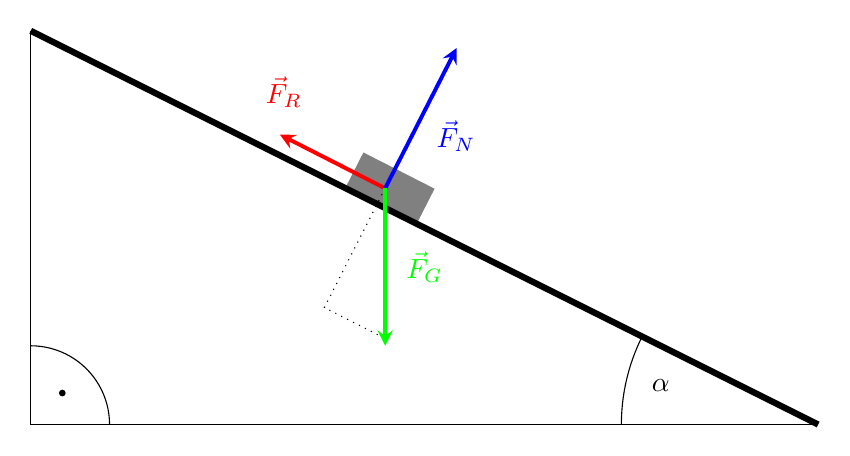
\begin{tikzpicture}
    \draw [fill, gray, rotate around={-27:(4,3)}](4,3) rectangle (5,3.5);
    \draw   (0,5) -- (0,0) -- (10,0);
    \draw [line width=0.8mm](0,5) -- (10,0);
    \draw  [domain=0:90] plot ({cos(\x)}, {sin(\x)});
    \draw [fill](0.4,0.4) circle (1pt);
    \draw [domain=153:180] plot ({10+2.5*cos(\x)}, {2.5*sin(\x)});
    \draw (8,0.5) node {$\alpha$};
    \draw [-stealth, red, line width=0.5mm, rotate around={-27:(4.5,3)}](4.5,3)--(3,3);
    \draw [red, rotate around={-27:(4.5,3)}](2.8,3.5) node {$\vec{F}_{R}$};
    \draw [-stealth, blue, line width=0.5mm, rotate around={-27:(4.5,3)}](4.5,3)--(4.5,5);
    \draw [blue, rotate around={-27:(4.5,3)}](5,4) node {$\vec{F}_{N}$};
    \draw [dotted, rotate around={-27:(4.5,3)}](4.5,3)--(4.5,1.3)--(5.4,1.3);
    \draw [-stealth, green, line width=0.5mm](4.5,3)--(4.5,1);
    \draw [green](5,2) node {$\vec{F}_{G}$};
\end{tikzpicture}
    \caption[Kräfte]{Kräfte, die auf den Körper Wirken}
    \label{fig:Kräfte}
\end{figure}

$\vec{F}_G$ lässt sich in eine zur Ebene parallele und eine senkrechte Komponente unterteilen. Die senkrechte Komponente von $\vec{F}_G$ wird durch $\vec{F}_N$ kompensiert, da $\vec{F}_N$ die selbe Kraft senkrecht zur Ebene nach oben auf den Körper ausübt wie $\vec{F}_G$ senkrecht zur Ebene nach unten. Der zur Ebene parallele teil von $\vec{F}_G$ wird als Hangabtriebskraft $\vec{F}_{HA}$ bezeichnet. $\vec{F}_R$ wirkt in Tangentialrichtung und hemmt somit die Bewegung des Körpers.\newline
Da für $\vec{F}_{G} = m \cdot \vec{g}$ gilt, gilt ebenfalls:

\begin{align}
    \abs{\vec{F}_{N}} = m \cdot g \cdot \cos{\alpha} \label{eq:F_N} \\
    \abs{\vec{F}_{HA}} = m \cdot g \cdot \sin{\alpha} \label{eq:F_HA}
\end{align}

wobei $\alpha$ der Neigungswinkel der Ebene ist.
Es kann zwischen Haftreibung, Gleitreibung und Rollreibung unterschieden werden, wobei sich in diesem Versuch nur auf Haft- und Gleitreibung fokusiert wird.
\newline
Solange der Körper sich nicht bewegt wird $\vec{F}_{HA}$ komplett durch die Haftreibung $\vec{F}_{HR}$ kompensiert. $\vec{F}_{HR}$ gilt immer dann, wenn sich zwei Flächen berühren und nicht gleiten. $\vec{F}_{HR}$ kann dabei $\abs{\vec{F}_{HR}^{max}}$ nicht überschreiten:
\begin{subequations}
    \begin{align}
        \abs{\vec{F}_{HR}^{max}} &= \mu_{HR} \cdot \abs{\vec{F}_{N}} \text{ bzw.}\\
        \abs{\vec{F}_{HR}} &\leq \mu_{HR} \cdot \abs{\vec{F}_{N}}
    \end{align}
    \label{eq:F_HR}
\end{subequations}
$\mu_{HR}$ hängt von Materialien, der Oberflächenbeschaffenheiten, sowie der Temperatur ab. \newline

Sobald $\vec{F}_{HA}$ größer als $\abs{\vec{F}_{HR}^{max}}$ wird fängt der Körper an zu gleiten und es gilt die Gleitreibung $\vec{F}_{GR}$:
\begin{align}
    \abs{\vec{F}_{GR}} = \mu_{GR} \cdot \abs{\vec{F}_{N}}
    \label{eq:F_GR}
\end{align}
$\mu_{GR}$ ist typischerweise kleiner als $\mu_{HR}$. Es wird angenommen, dass $\vec{F}_{R}$ bei einer trockenen Oberfläche unabhängig von der Geschwindigkeit des Körpers ist.\smallskip

Die resultierende Gesamtkraft $\vec{F}_{res}$ (siehe \autoref{fig:Gesamtkraft}) wird nach Newtons zweiten Axiom, dass die Kraft gleich die Masse mal die Beschleunigung ist:
\begin{align}
    \vec{F}_{res} = \vec{F}_{HA} + \vec{F}_{GR} = m \cdot \vec{a}
\end{align}

\begin{figure}[ht]
    \centering
    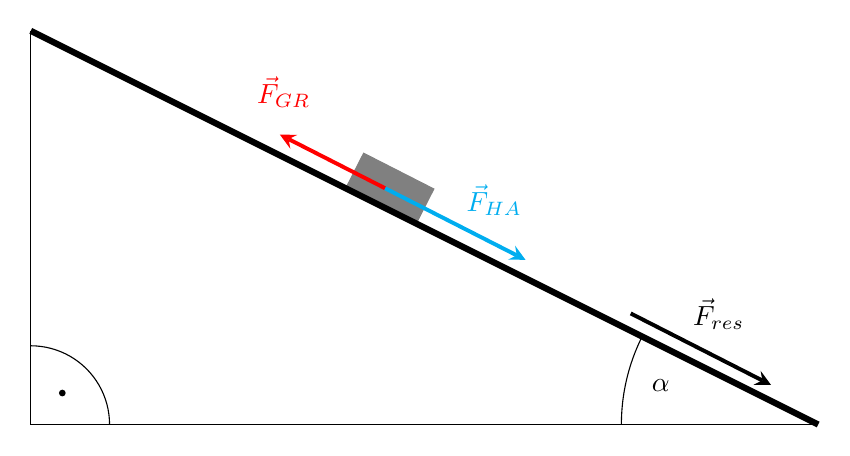
\begin{tikzpicture}
    \draw [fill, gray, rotate around={-27:(4,3)}](4,3) rectangle (5,3.5);
    \draw   (0,5) -- (0,0) -- (10,0);
    \draw [line width=0.8mm](0,5) -- (10,0);
    \draw  [domain=0:90] plot ({cos(\x)}, {sin(\x)});
    \draw [fill](0.4,0.4) circle (1pt);
    \draw [domain=153:180] plot ({10+2.5*cos(\x)}, {2.5*sin(\x)});
    \draw (8,0.5) node {$\alpha$};
    \draw [-stealth, red, line width=0.5mm, rotate around={-27:(4.5,3)}](4.5,3)--(3,3);
    \draw [red, rotate around={-27:(4.5,3)}](2.8,3.5) node {$\vec{F}_{GR}$};
    \draw [-stealth, cyan, line width=0.5mm, rotate around={-27:(4.5,3)}](4.5,3)--(6.5,3);
    \draw [cyan, rotate around={-27:(4.5,3)}](5.8,3.5) node {$\vec{F}_{HA}$};
    \draw [line width=0.5mm, -stealth, rotate around={-27:(4.5,3)}] (8,3) -- (10,3);
    \draw [rotate around={-27:(4.5,3)}](9,3.5) node {$\vec{F}_{res}$};
\end{tikzpicture}
    \caption[Resultierende Gesamtkraft]{Aus $\vec{F}_{GR}$ und $\vec{F}_{HA}$ resultierende Gesamtkraft $\vec{F}_{res}$}
    \label{fig:Gesamtkraft}
\end{figure}

Die Beschleunigung $a$ wird als Funktion der zurückgelegten Strecke $l$ und der benötigten Zeit $t_{mess}$ ausgedrückt, da gilt:
\begin{align}
    l = \frac{1}{2} a \cdot t_{mess}^2
\end{align}
Bei berücksichtigung der Formeln \autoref{eq:F_N} und \autoref{eq:F_GR}, ist es möglich den $\mu_{GR}$ zu bestimmen:
\begin{align}
    \mu_{GR} = \tan{a} - \frac{2\cdot l}{g \cdot t_{mess}^2 \cdot \cos{a}}
\end{align}
    \newpage

    \section{Versuchsaufbau}

Für den Versuch wird ein Gerüst benutzt, welches ein glattes Brett hält und ermöglicht den Winkel zwischen der horizontalen Ebene und dem Brett einzustellen. An beiden Enden des Bretts befindet sich jeweils eine Lichtschranke, welche sich verschieben lassen.\\
Ein Holzquader mit vier unterschiedlichen Oberflächen wird auf das glatte Brett gelegt. Eine Seite des Quaders ist unbeschichtet, eine ist mit Gummi beklebt, auf einer ist Klebeband und die letzte Seite ist lackiert. Der Quader rutscht über das Brett, sobald der Winkel hoch genug ist.\\
Ebenfalls wird ein Gliedermaßstab, um die Länge $l$ zwischen den Lichtschranken zu messen, und ein Winkelmesser, mit dem $\alpha$ berechnet wird, gebraucht.
\begin{figure}[ht]
    \centering
    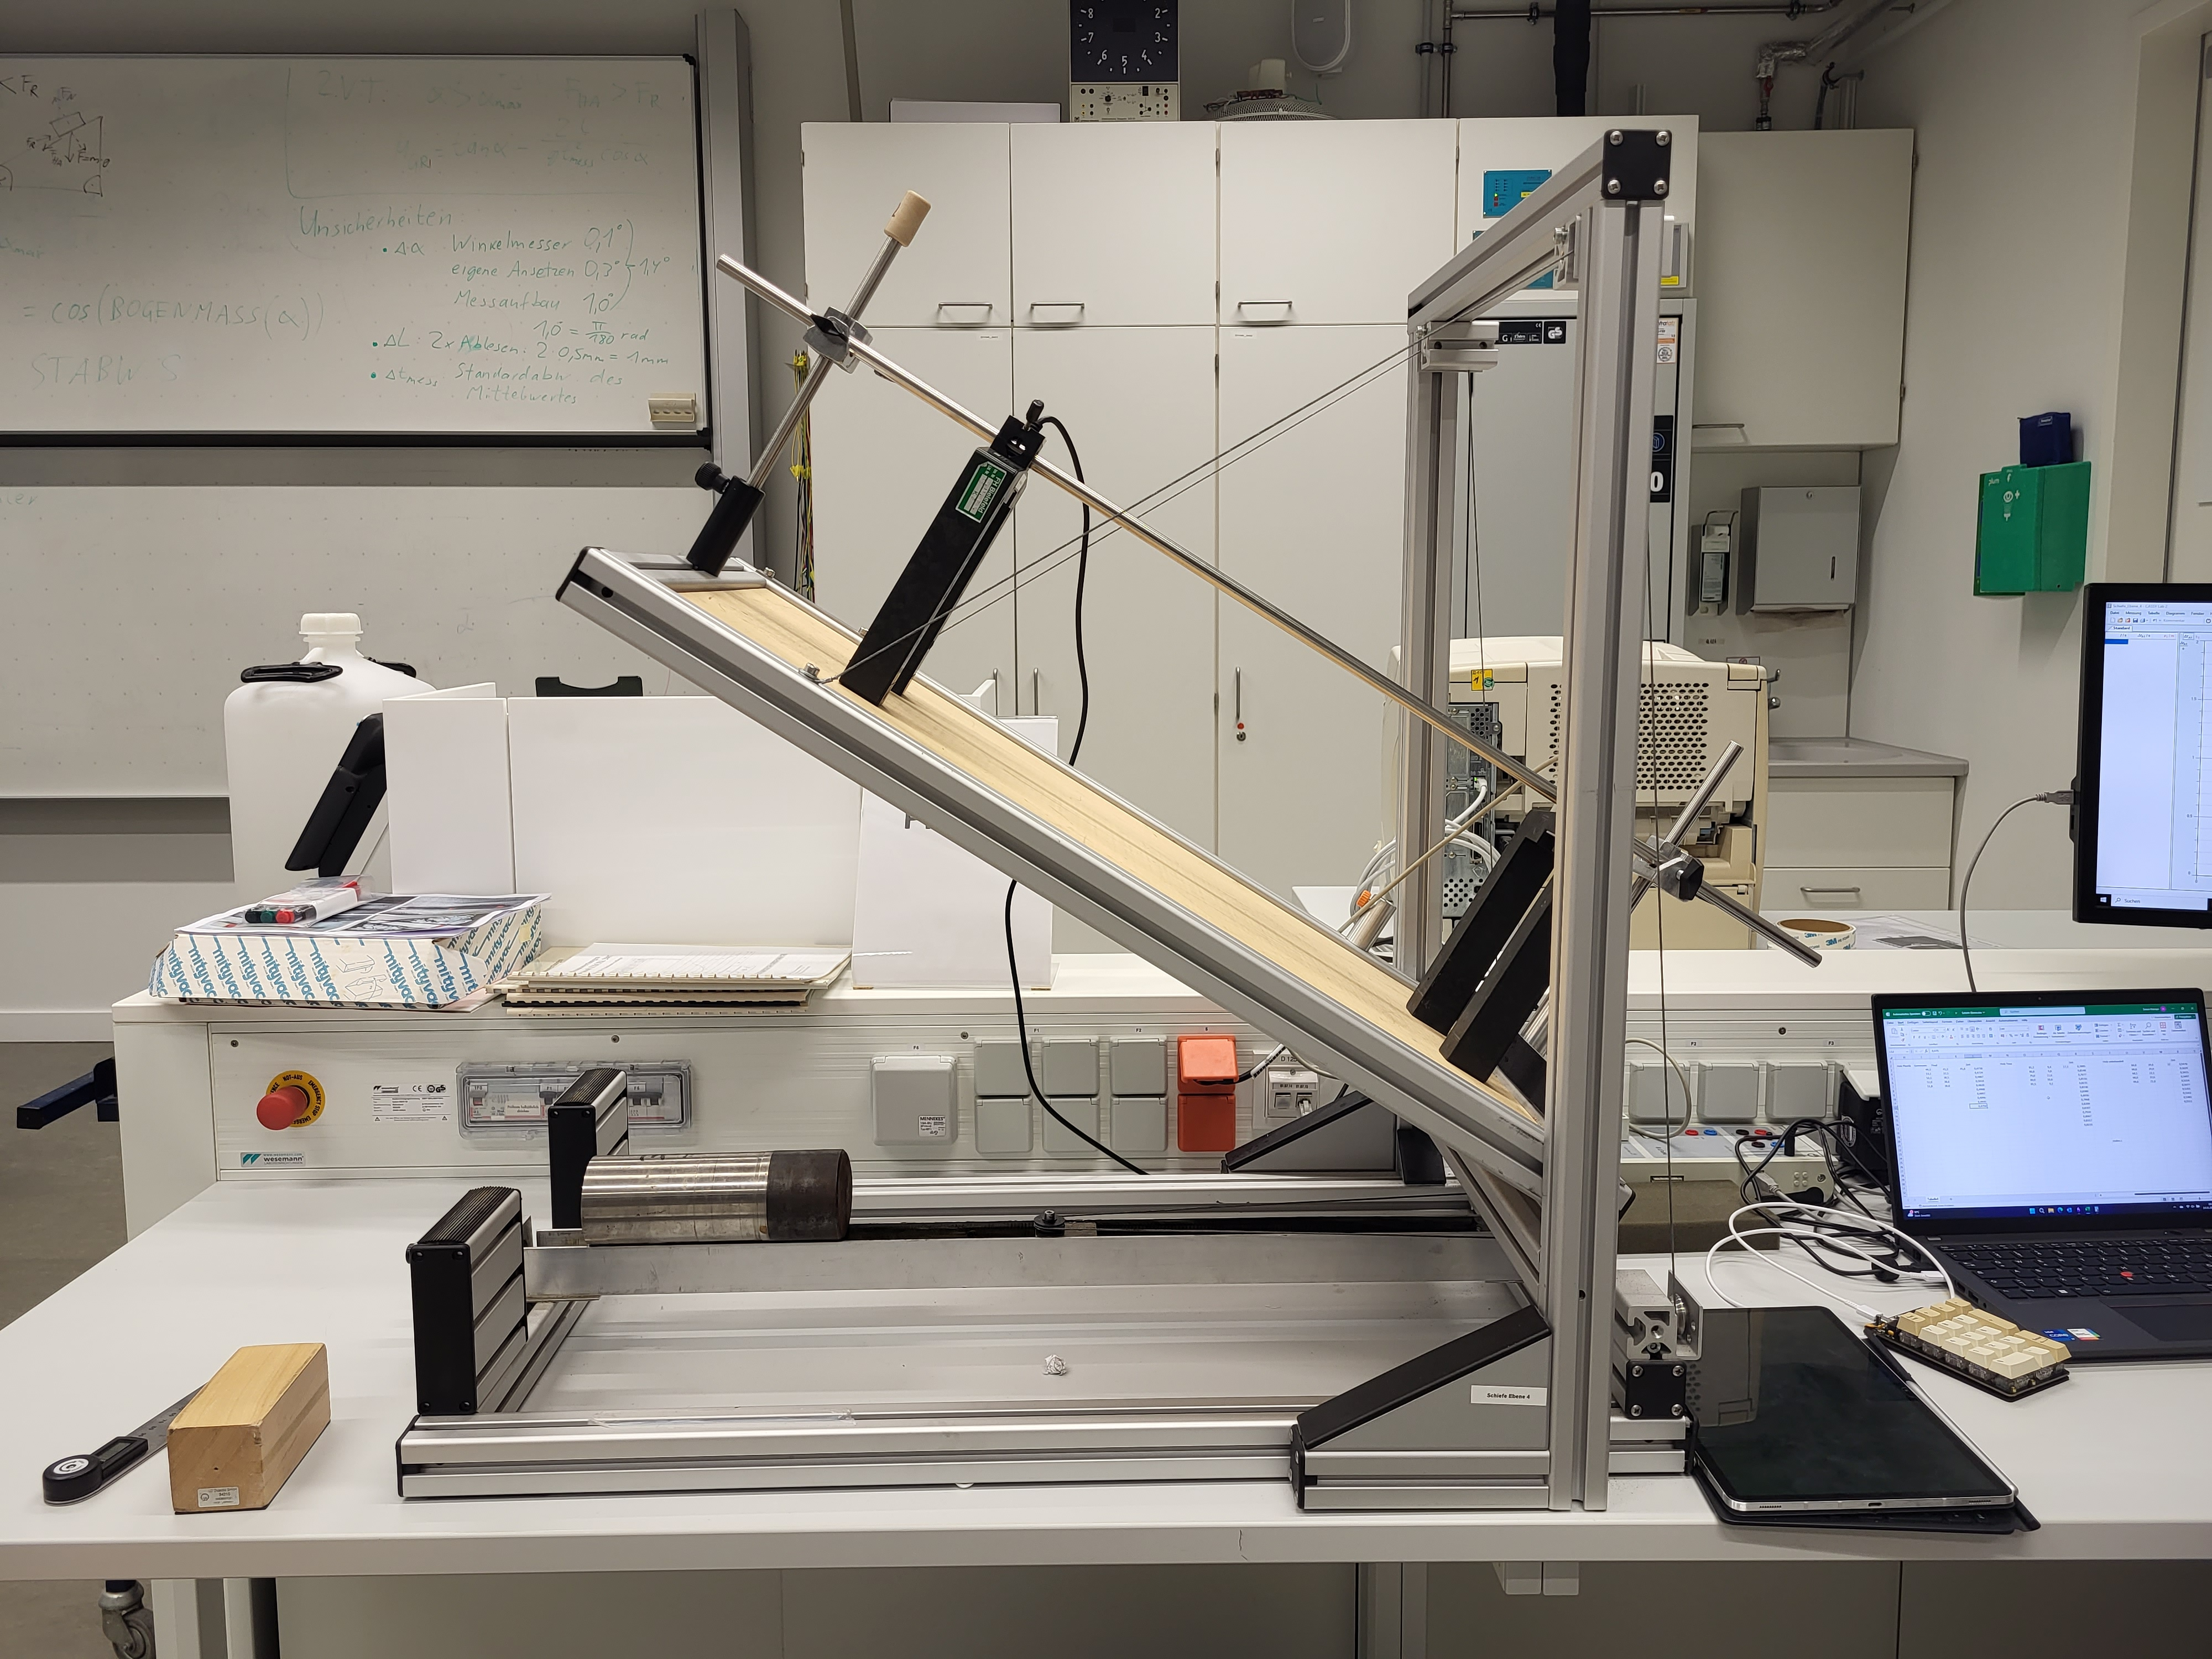
\includegraphics[width=\linewidth/2]{images/Versuch-Aufbau.jpg}
    \caption[Aufbau]{Gerüst mit glattem Brett und Lichtschranken}
    \label{fig:Aufbau}
\end{figure}
    \newpage

    \input{src/Versuchsdurchführung}
    \newpage

    \section{Messdaten}

Zunächst erfolgt die Darstellung der Messergebnissem um auf deren Basis die Haftreibungskoeffizienten $\mu_{HR}$ und Gleitreibungskoeffizienten $\mu_{GR}$ für die drei Oberflächenmaterialien X, Y, und Z zu bestimmen.

\subsection{Messungen zur Haftreibung}

\subsection{Messungen zur Gleitreibung}

\subsubsection{Zurückgelegte Strecke des Körpers}

\subsubsection{Eingestellter Winkel}

\subsubsection{Gemessene Zeit $t_{mess}$}
    \newpage

    \section{Versuchsauswertung}

Test  Test Test

\subsection{Bestimmung des Haftreibungskoeffizienten}

Im Folgenden werden die Berechnungen zur Bestimmung des Haftreibungskoeffizienten $\mu_{HR}$ durchgeführt.

\subsubsection{Statistische Auswertung des Winkels}

Die in \autoref{tab:maximalerNeigungswinkel} gemessenen Werte werden für die weitere Arbeit statistisch Ausgewertet. Dazu wird der Mittelwert $\bar{\alpha}_{max}$, die Standardabweichung der Stichprobe $\sigma_{n-1}$ und die Standardabweichung des Mittelwertes $\sigma_{\alpha}$ berechnet.

In \autoref{tab:statWinkel} sind die Ergebnisse der statischen Auswertung zu sehen.

\begin{table}[h]
    \center 
    \caption[Statistische Auswertung des maximalen Neigungswinkels]{Ergebnisse der statischen Auswertung des maximalen Neigungswinkels}
    \begin{tabular}{c|c|c|c}
    \space & Oberfläche X & Oberfläche Y & Oberfläche Z \\ \hline
    $\bar{\alpha}_{max}$ & 38,94 & 10,10 & 22,86 \\
    $\sigma_{n-1}$ & 1,411737 & 1,009950 & 1,451895 \\
    $\sigma_{\bar{\alpha}}$ & 0,631348 & 0,451664 & 0,649307 \\
\end{tabular}
    \label{tab:statWinkel}
\end{table}

\subsubsection{Berechnung des Haftreibungskoeffizienten und Größtfehlers}

Die Haftreibungskraft $\vec{F}_{HR}$ wirkt dann, wenn sich der Körper nicht bewegt. Da er sich nicht bewegt, kompensiert $\vec{F}_{HR}$ die Hangabtriebskraft $\vec{F}_{HA}$. Die Haftreibungskraft hat einen maximalen Wert von $\vec{F}_{HR}^{max}$, welche Sie nicht überschreiten kann. Daher kann mit \autoref{eq:F_HR}, \autoref{eq:F_HA} und der \autoref{fig:Kräfte}, $\mu_{HR}$ hergeleitet werden.

\begin{align*}
  \abs{\vec{F}_{HR}^{max}} = \abs{\vec{F}_{HA}} &= \mu_{HR} \cdot \abs{\vec{F}_{N}} \quad \text{mit} & \abs{\vec{F}_{HA}} = m \cdot g \cdot \sin(\alpha_{max}) \, , \, \abs{\vec{F}_{N}} &= m \cdot g \cdot cos(\alpha_{max})
\end{align*}
\vspace{-1cm}
\begin{alignat}{3}
  &\Rightarrow &\quad m \cdot g \cdot \sin(\alpha_{max}) &= \mu_{HR} \cdot m \cdot g \cdot cos(\alpha_{max}) \nonumber \\
  &\Leftrightarrow &\quad \frac{m \cdot g \cdot \sin(\alpha_{max})}{m \cdot g \cdot \cos(\alpha_{max})} &= \mu_{HR}\nonumber \\ 
  &\Leftrightarrow &\quad \tan(\alpha_{max}) &= \mu_{HR} \label{eq:muHR}
\end{alignat}

wobei $\alpha_{max}$ der größte Winkel ist, bei dem der Körper noch ruht.\newline

Da $\mu_{GR}$ mit gemessenen Werten berechnet wird, muss einee Größtfehlerbetrachtung gemacht werden. Dafür gilt:


\begin{align}
\mu_{\mathrm{HR}} &=\tan \left(\alpha_{\max }\right) \quad \Rightarrow \nonumber \\
\Delta \mu_{\mathrm{HR}}&=\left|\frac{\partial \mu_{\mathrm{HR}}}{\partial \alpha_{\max }} \cdot \Delta \alpha_{\max }\right|=\abs*{\frac{1}{\cos ^{2}\left(\alpha_{\max }\right)} \cdot \Delta \alpha_{\max }} \label{eq:DeltaMuHR}
\end{align}
\begin{conditions}
\alpha_{max} & maximaler Neigungswinkel. Angegeben im Bogenmaß.
\end{conditions}

In \autoref{tab:muGRWerte} wird mit \autoref{eq:DeltaMuHR} und \autoref{eq:muHR}, $\mu_{HR}$ und $\Delta \mu_{HR}$ für alle drei Oberflächen berechnet.

\begin{table}[h]
  \center 
  \caption[Haftreibungskoeffizienten und Größtfehler]{Ergebnisse der Berechnung des Haftreibungskoeffizienten $\mu_{HR}$ und Größtfehlers}
  \begin{tabular}{c|c|c|c}
    \space & Oberfläche X & Oberfläche Y & Oberfläche Z \\ \hline
    $\mu_{GR}$ & 0,808052 & 0,178127 & 0,421594 \\
    $\Delta \mu_{GR}$ & 0,018214 & 0,008133 & 0,013347
\end{tabular}
  \label{tab:muGRWerte}
\end{table}

\subsubsection{Angabe des Endergebnisses}

In \autoref{tab:EndergebnissMuHR} erfolgt die Angabe des Endergebnisses für den Haftreibungskoeffizienten $\mu_{HR}$.

\begin{table}[h]
  \center 
  \caption[Endergebnisse des Haftreibungskoeffizienten]{Angabe des Endergebnisses für den Haftreibungskoeffizienten $\mu_{HR}$}
  \begin{tabular}{c|ccc}
    Oberfläche & $\mu_{HR}$ & $\pm$ & $\Delta \mu_{HR}$ \\ \hline
    X & 0,808 & $\pm$ & 0,019 \\
    Y & 0,178 & $\pm$ & 0,009 \\
    Z & 0,422 & $\pm$ & 0,014
\end{tabular}
  \label{tab:EndergebnissMuHR}
\end{table}
\subsection{Bestimmung des Gleitreibungskoeffizienten}

\subsubsection{Statistische Auswertung der gemessenen Zeit}

Die in \autoref{tab:gemesseneZeit} gemessenen Werte werden für die weitere Arbeit statistisch Ausgewertet. Dazu wird der Mittelwert $\bar{t}_{mess}$, die Standardabweichung der Stichprobe $\sigma_{n-1}$ und die Standardabweichung des Mittelwertes $\sigma_{\bar{t}}$ berechnet.

In \autoref{tab:statZeit} sind die Ergebnisse der statischen Auswertung zu sehen.

\begin{table}[h]
    \center 
    \caption[Statistische Auswertung der gemessenen Zeit]{Ergebnisse der statischen Auswertung der gemessenen Zeit}
    \begin{tabular}{c|c|c|c}
    \space & Oberfläche X & Oberfläche Y & Oberfläche Z \\ \hline
    $\bar{t}_{mess}$ & 0,485730 & 0,813020 & 0,545010 \\
    $\sigma_{n-1}$ & 0,009620 & 0,026040 & 0,019323 \\
    $\sigma_{\bar{t}}$ & 0,003042 & 0,008235 & 0,006111 
\end{tabular}
    \label{tab:statZeit}
\end{table}

\subsubsection{Berechnung des Gleitreibungskoeffizienten und Größtfehlers}

Die Gleitreibungskraft $\vec{F}_{GR}$ wirkt, wenn sich der Körper bewegt. Sie ist kleiner als die Haftreibungskraft $\vec{F}_{HR}$. Aus \autoref{fig:Gesamtkraft} und \autoref{eq:F_N} und \autoref{eq:F_GR} kann somit $\mu_{GR}$ bestimmt werden.

\begin{align}
  \mu_{GR} = \tan{a} - \frac{2\cdot l}{g \cdot t_{mess}^2 \cdot \cos{a}}
  \label{eq:muGR}
\end{align}

Da $l$ und $t_{mess}$ gemessen werden, muss eine Größtfehlerbetrachtung gemacht werden. Dafür gilt:

\begin{align}
  \mu_{GR} = tan(\alpha) - \frac{2 \cdot l}{g \cdot \bar{t}_{mess}^2 \cdot \cos(\alpha)} \quad \Rightarrow
\end{align}
\begin{equation}
  \begin{alignedat}{2}
    \Delta \mu_{GR} &= &\quad \abs*{\frac{\partial \mu_{GR}}{\partial l} \cdot \Delta l}_{\bar{t}_{mess},\alpha = konst.} + \abs*{\frac{\partial \mu_{GR}}{\partial \bar{t}_{mess}} \cdot \Delta \bar{t}_{mess}}_{l,\alpha = konst.} + \abs*{\frac{\partial \mu_{GR}}{\partial \alpha} \cdot \alpha}_{\bar{t}_{mess},l = konst.}\\
    &= &\, \abs*{-\frac{2}{g \cdot \bar{t}_{mess}^2 \cdot \cos(\alpha)}\cdot \Delta l}_{\bar{t}_{mess},\alpha = konst.} + \abs*{\frac{4 \cdot l}{g \cdot \bar{t}_{mess}^2 \cdot \cos(\alpha)} \cdot \Delta \bar{t}_{mess}}_{l,\alpha = konst.} \\ 
    &\quad  &+ \, \abs*{\frac{1}{\cos^2( \alpha )} -\frac{2 \cdot l \cdot \sin(\alpha)}{g \cdot \bar{t}_{mess}^2 \cdot \cos^2(\alpha)} \cdot \Delta \alpha}_{\bar{t}_{mess},l = konst.}
  \end{alignedat}
  \label{eq:DeltaMuGR}
\end{equation}
\begin{conditions}
  \bar{t}_{mess} & Mittelwert der einzelnen Messungen. \autoref{tab:statZeit}\\
  \Delta \bar{t}_{mess} & Standardabweichung des Mittelwertes. \autoref{tab:statZeit}\\
  \alpha & Eingestellter Winkel in Bogenmaß.
\end{conditions}

In \autoref{tab:EndergebnissMuGR} werden die Gleitreibungskoeffizienten $\mu_{GR}$ und Größtfehlerbetrachtung, mit \autoref{eq:muGR} und \autoref{eq:DeltaMuGR}, für alle drei Oberflächen gemacht.

\begin{table}[h]
  \center 
  \caption[Endergebnisse des Gleitreibungskoeffizienten]{Angabe des Endergebnisses für den Gleitreibungskoeffizienten $\mu_{GR}$}
  \begin{tabular}{c|ccc}
    Oberfläche & $\mu_{HR}$ & $\pm$ & $\Delta \mu_{HR}$ \\ \hline
    X & 0,38 & $\pm$ & 0,04 \\
    Y & 0,141 & $\pm$ & 0,021 \\
    Z & 0,198 & $\pm$ & 0,029
\end{tabular}
  \label{tab:EndergebnissMuGR}
\end{table}

\subsubsection{Angabe des Endergebnisses}
\subsection{Diskussion} \label{chap:Diskussion}
Mehrere Variablen haben bei diesem Versuch einen Einfluss auf das Ergebnis, wobei sich nur wenige davon kontrollieren lassen. Die am einfachsten zu kontrollierende Variable ist die Länge $l$ zwischen den beiden Lichtschranken.
\\
Diese Erhöhung kann zu einem genaueren Ergebnis führen, weil sich somit der Messfehler von $l$ prozentual verringert. Ein weiterer Vorteil von einer höheren Länge ist, dass Fehler, wie eine leichte Startgeschwindigkeit des Körpers, auf die erhöhte Länge betrachtet, einen geringeren Einfluss haben. \\ $l$ kann allerdings auch nicht beliebig angehoben werden, da der Körper nicht immer in einer graden Linie auf der Ebene hinunterrutscht und somit das Ergebnis verfälschen kann. Ebenfalls kann dieses schiefe Rutschen dazu führen, dass der Körper die untere Lichtschranke garnicht trifft und somit garkeine Messung stattfindet und die jeweilige Messung wiederholt werden muss.\bigbreak 
Eine weitere Möglichkeit genauere Ergebnisse zu erhalten ist den Winkel $\alpha$ genauer zu messen und ihn zwischen Messungen genauer zu halten, da es bei dem aktuellen Aufbau sein kann, dass sich $\alpha$ minimal verschiebt. Dies ist ein Problem, da immer mit dem selben Winkel gerechnet wird und eine leichte Verstellung die ohnehin schon hohe Messunsicherheit weiter erhöht. \\ 
$\alpha$ ist mit einer Messunsicherheit von $\Delta \alpha = 0,9^\circ$ hoch und eine Möglichkeit zur genaueren Messung kann ebenfalls einen positiven Einfluss auf die genauigkeit des Ergebnisses haben.
    \newpage

    \section{Zusammenfassung und Ausblick}

Wie in \autoref{chap:Diskussion} beschrieben wird, gibt es viele Möglichkeiten genauere Ergebnisse für $\mu_{HR}$ und $\mu_{GR}$ zu erhalten. Es ist auch zu erkennen, dass sich die Haftreibungskoeffizienten $\mu_{HR}$ und Gleitreibungskoeffizienten $\mu_{GR}$ mit den unterschiedlichen Oberflächenmaterialien ändern. Dabei kann erkannt werden, dass die koeffizienten von der Härte des Materials abhängig sind. Gummi hat jeweils die größten koeffizienten und lackiertes Holz, welche härter ist, besitzt die kleinsten koeffizienten.

Ebenfalls wird erkannt, dass genauere Messergebnisse mit homgenen Oberflächen erzielt werden. Dies lässt sich an dem Besipiel von der mit Klebeband beschichteten Blockseite erkennen, da das Klebeband uneben abgenutzt ist und somit keine homogene Fläche gegeben ist. Das hat zur Folge, dass der Block nicht gerade an der schiefen Ebene herunterrutscht, sondern anfängt schief zu rutschen, da unterschiedliche Reibungen an unterschiedlichen Stellen der Oberfläche wirken. Die länge ist somit nicht mehr eindeutig zu bestimmen und variiert bei jeder Durchführung.
    \newpage

    %Literaturverzeichnis
    %\bibliographystyle{gerabbrv}
    %\bibliography{src/literatur}
    %\newpage

    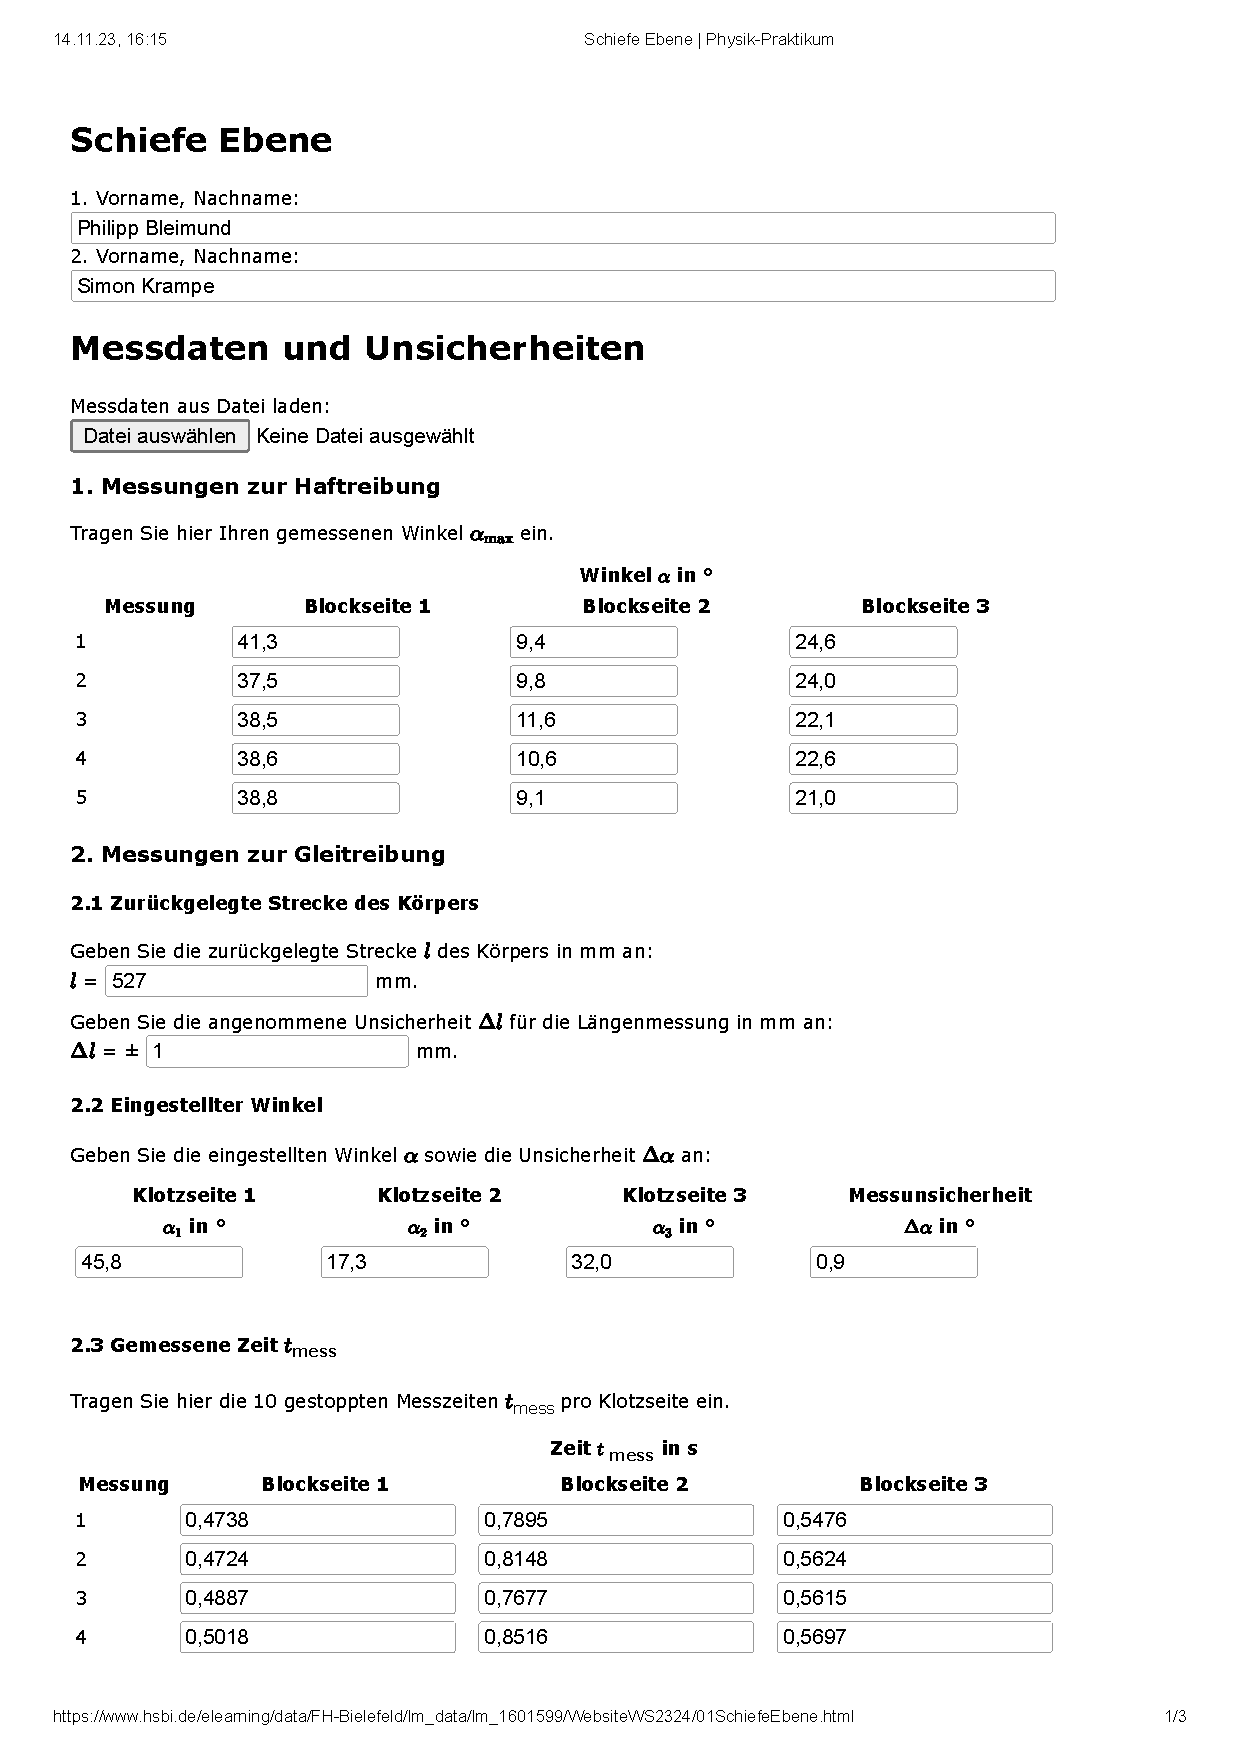
\includepdf[pages={1,2,3}]{src/Schiefe_Ebene___Physik-Praktikum.pdf}

    \clearpage
\end{document}